%\subsection*{Statement of authorship}
\renewcommand{\arraystretch}{1.5}
\begin{tabular}{m{0.25\textwidth} m{0.67\textwidth}}
    \hline \hline Paper title & A non-iterative method to solve for magnetic fields, forces, and torques due to permanent magnets with non-unity relative permeability \\ \hline
    Publication status & Submitted \\ \hline
    Publication details & Submitted to \textit{Journal of Magnetism and Magnetic Materials}, Dec. 2021 \\ \hline \hline
\end{tabular}

\vfill

\subsection*{Principal author}
\begin{tabular}{p{0.25\textwidth} m{0.67\textwidth}}
    \hline \hline Name & James O'Connell \\ \hline
    Contribution & \begin{itemize}
        \setlength\itemsep{-2mm}\small
        \item[-] Idea conceptualisation
        \item[-] Review of relevant literature
        \item[-] Deriving a matrix equation for the surface charge density of a magnet based on the field present and the remanence magnetisation of the magnet
        \item[-] Incorporating Gauss' Law for Magnetism into the system
        \item[-] Applying a constrained least squares methodology to solve an overdetermined matrix equation with constraints
        \item[-] Adapting the system of equations to include an arbitrary number of magnetic bodies and arbitrary external magnetic fields
        \item[-] Applied the surface charge density solution to find the magnetic field at any point
        \item[-] Applied the surface charge density solution to estimate the force and torque imparted on all magnets in the system
        \item[-] Implemented the surface charge, magnetic field, force, and torque methodologies in MATLAB code
        \item[-] Created finite element simulations to verify the algorithms and MATLAB code
        \item[-] Analysed the accuracy of the methodology based on mesh density
        \item[-] Wrote manuscript draft and created all figures
        \item[-] Finalisation of article
        \item[-] Preparation and submission for publication, including author correspondence
    \end{itemize} \\ \hline
    Percentage & 90\% \\ \hline
    Certification & \small This paper reports on original research conducted by the author during the period of Higher Degree by Research candidature and is not subject to any obligations or contractual agreements with a third party that would constrain its inclusion in this thesis. The author listed above is the primary author of this paper. \\ \hline
    Signature & \begin{tabular}{m{45mm} m{10mm} m{20mm}}
    \vspace{0.5mm}\includegraphics[width=0.3\textwidth]{jamesSignature.PNG} & Date: & 8 Dec 2021
    \end{tabular}
\end{tabular}

\vfill
    
\subsection*{Co-author contributions}
By signing this statement of authorship, each author certifies that:
\begin{enumerate}
    \item the candidate's stated contribution to the publication is accurate (as detailed above);
    \item permission is granted for the candidate to include the publication in the thesis; and
    \item the sum of all co-author contributions is equal to 100\% less the candidate's stated contribution.
\end{enumerate}
\begin{tabular}{m{0.25\textwidth} m{0.67\textwidth}}
    \hline \hline Name & Will Robertson \\ \hline
    Contribution & 5\% \\ \hline
    Signature & \vspace{2mm}\includegraphics[height=10mm]{willSig} \\  \hline
    Date & 16 Dec 2021 \\
    \hline \hline Name & Ben Cazzolato \\ \hline
    Contribution & 5\% \\ \hline
    Signature & \vspace{2mm} \includegraphics[height=10mm]{benSig} \\ \hline
    Date & 16 Dec 2021 \\
    \hline \hline \vfill
\end{tabular}
\renewcommand{\arraystretch}{1}
\newpage
%
\section*{\LARGE A non-iterative method to solve for magnetic fields, forces, and torques due to permanent magnets with non-unity relative permeability}
James L.G. O'Connell, William S.P. Robertson, and Benjamin S. Cazzolato
\section*{Abstract}\addcontentsline{toc}{section}{\protect\numberline{}Abstract}\label{sec:p4abstract}
Although the majority of common permanent magnet materials have relative permeabilities between 1.05 and 1.3, they are often modelled analytically with the assumption of unity relative permeability. While this greatly simplifies analysis, it introduces modelling errors, leading to overestimates of magnetic fields, forces, and torques. This paper presents a new method for modelling interactions between magnets with non-unity relative permeabilities assuming constant uniform remanence magnetisation and permeability. In contrast to other methods which use an iterative approach, this methodology requires calculating magnetic field information only once, leading to a considerable reduction in computational effort. Based on a triangular surface mesh, this method permits the calculation for any magnetic geometry and for magnetic systems with arbitrarily many magnets. Verification is performed using finite element simulations, with the proposed method showing high accuracy and speed.
\section{Introduction}\label{sec:p4introduction}
Magnetic materials are used in many applications found in science and engineering, including electric motors, loudspeakers, and magnetic data storage. Each material has a given magnetic relative permeability \(\mu_r\), which describes how the magnetisation of the material changes when magnetic fields are present. Most permanent magnet materials have a relative permeability slightly larger than unity, but are often modelled with \(\mu_r = 1\), ignoring the effect of permeability. This significantly decreases the complexity of modelling, but introduces errors as the magnitude of permeability increases. Some materials such as iron have a high permeability, and are often modelled by assuming the permeability is infinite, also leading to modelling errors. To reduce these modelling errors, non-unity finite permeability must be considered, but this is difficult to model and analyse, often requiring the use of finite element simulations or iterative solvers.

Several researchers have attempted to analytically model magnetic permeability with varying levels of success. \textcite{Kremers2013} modelled a permanent magnet with non-unity permeability by modifying the magnetisation strength of the magnet based on the permeability. This approach gives extremely fast results for the magnetic field produced by a single magnet with low permeability. However, it does not consider the effect of external fields or magnets, and is only valid for small and constant permeabilities, limiting accuracy. \textcite{Dam2016} extended upon this by calculating the interaction force in two of the three Cartesian directions as one magnet is rotated with non-unity relative permeability. However, the third force component was not derived, and the methodology is only valid for cuboidal magnets. \textcite{Casteren2014} published a more general iterative methodology applicable to any magnet geometry, which was more accurate at the cost of considerably longer calculation times. Their approach assumed constant permeability and required recalculating the magnetic field for each iteration, but could incorporate external fields and arbitrarily large permeabilities. In a recent study, \textcite{Zhang2021} performed a similar analysis by subdividing cuboidal permanent magnets into a large number of smaller cuboidal magnets, with the magnetisation of each augmented by the effects of permeability. The force equations from \textcite{Akoun1984}, which assume unity relative permeability, were implemented on each small cuboid, giving accurate force calculations which incorporate the effect of permeability. \textcite{Forbes2021} also subdivided magnetic materials into smaller volumes of material with similar outcomes. Provided the permeability of each segment remains uniform across its volume, the permeability within each sub-volume was able to vary, allowing the modelling of nonlinear magnetic materials.

\textcite[Sec~2.6]{Harrington1993} presented an interesting methodology in electrostatics, wherein the polarisability of a dielectric body is calculated under the assumption of non-unity relative electric permittivity. This is analogous to finding the magnetisation of a magnetic body with non-unity relative permeability, but in the electrostatic domain rather than the magnetostatic. Their method is based on solving a matrix equation based on electric surface charges and the permittivity of the material, allowing a solution to be found. However, their method uses approximations of the integral equations for the field, leading to small but non-trivial errors in the solution.

The current paper introduces a new methodology for calculating magnetic fields, forces, and torques due to magnetic materials with non-unity permeabilities in a single step, thus avoiding iteration. It is similar in concept to the aforementioned matrix equation given by \textcite[Sec~2.6]{Harrington1993}, but with several advantages. The method presented in this paper uses the exact solution to the field equations, leading to high accuracy. In addition, a constraint is applied to the system to ensure consistency with Gauss' Law for Magnetism, further increasing accuracy. Furthermore, systems with arbitrarily many magnets and systems with external field sources may be analysed with this method. Finally, the methodology presented in this paper includes the evaluation of forces and torques on magnetic bodies through numeric integration, allowing analysis of quasi-static magnetic systems.

This methodology is extremely fast and gives accurate results for any magnet shape due to the use of a triangular surface mesh. The methodology begins by calculating surface charge densities in Section \ref{sec:p4magneticChargeDensity}, before using these results to calculate magnetic fields (Section \ref{sec:p4magneticField}), as well as forces and torques (Section \ref{sec:p4forceAndTorque}). Verification is performed on this methodology using several magnetic configurations in Section \ref{sec:p4verification}. Finally, computational considerations are detailed in Section \ref{sec:p4computationalPerformance} before the paper is concluded.
\section{Magnetic charge density}\label{sec:p4magneticChargeDensity}
To calculate the effect of magnetic permeability on magnetic materials, this paper uses the magnetic charge model \cite{Furlani2001}, where fictitious magnetic charges exist on the surface of and inside magnetic bodies. An example of this is depicted in Figure \ref{fig:p4singleMagnetPicture}, where an idealised permanent magnet with unity relative permeability \(\mu_r = 1\) and a non-ideal permanent magnet with \(\mu_r = 3\) have been drawn, with positive charges shown in red and negative charges in blue. Both magnets have identical remanence magnetisations, but the non-ideal magnet has a demagnetising effect on itself due to a relatively large value of permeability, resulting in weaker surface charges and some charges migrating from the north and south poles to the sides of the magnet. For non-unity relative permeability, the distributions of magnetic charge on the magnet surfaces is unknown and must be solved based on their interaction with each other and any applied magnetic field. This section outlines an approach to calculating these charge densities which uses a one-step matrix inversion rather than the iterative approach commonly seen in literature.
\begin{figure}
    \centering
    \begin{subfigure}{0.7\textwidth}
        \centering
        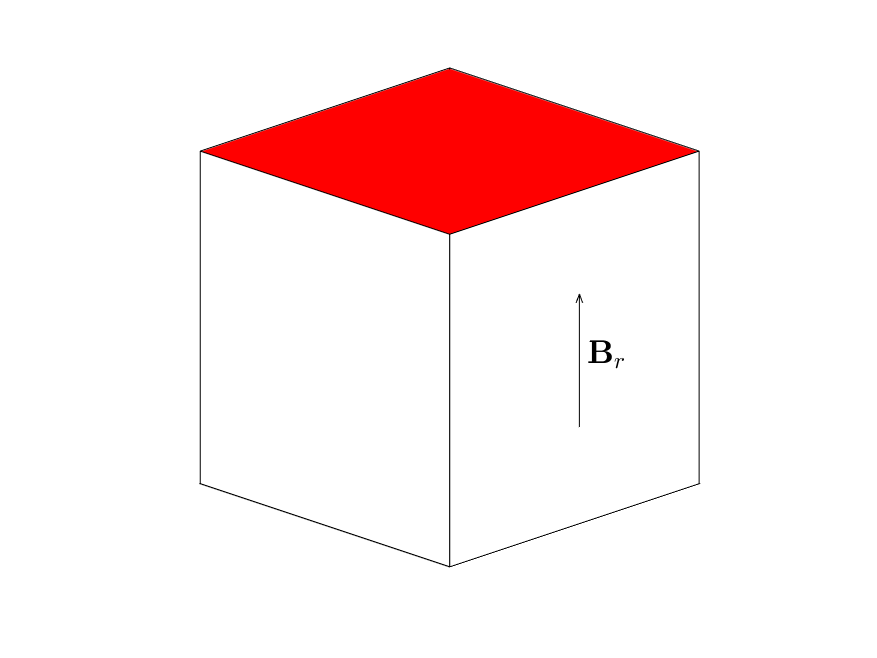
\includegraphics[width=\linewidth]{p4/p4FIG1a}
        \caption{}\label{fig:p4singleMagnetIdealised}
    \end{subfigure}
    \begin{subfigure}{0.7\textwidth}
        \centering
        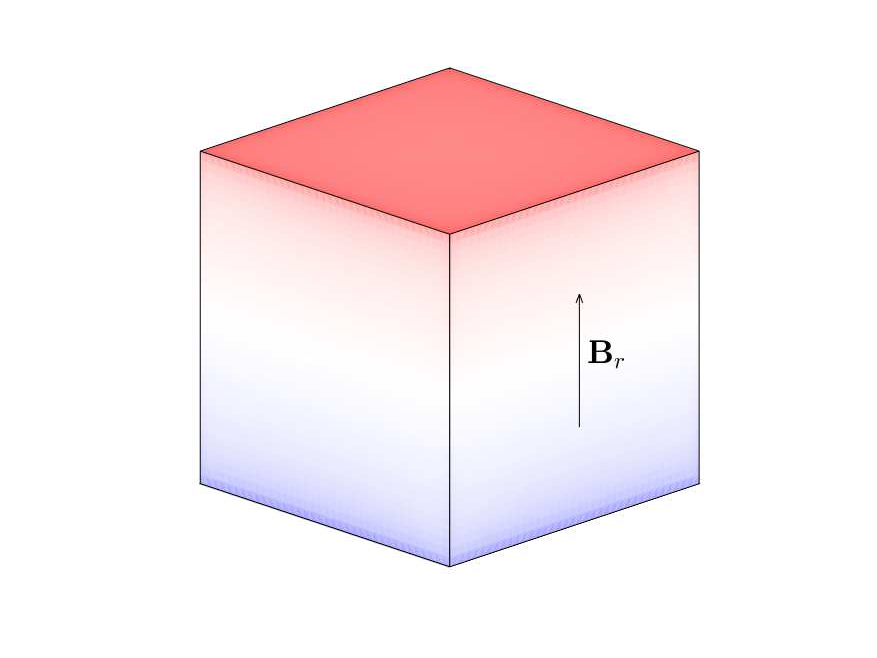
\includegraphics[width=\linewidth]{p4/p4FIG1b}
        \caption{}\label{fig:p4singleMagnetNonideal}
    \end{subfigure}
    \caption{A cube magnet with an ideal relative permeability \(\mu_r = 1\) (a) and a non-ideal relative permeability \(\mu_r = 3\) (b). The remanence magnetisation of both magnets is equal in strength and in the vertical direction, with the associated surface charges shown in red (positive charge) and blue (negative charge). The surface charges on the idealised magnet (\(\mu_r = 1\)) remain on the poles, whereas the charges on the non-ideal magnet (\(\mu_r = 3\)) migrate from the poles and become weaker due to the self-demagnetising effect of relatively large permeability.}
    \label{fig:p4singleMagnetPicture}
\end{figure}
%
\subsection{Induced magnetisation and surface charge density}
At any point in space, magnetic materials satisfy the constitutive relationship
\begin{equation}\label{eqn:p4constitutiveRelation}
    \mathbf{B} = \mu_0 \left( \mathbf{H} + \mathbf{M} \right)
\end{equation}
and Gauss' law for magnetism
\begin{equation}\label{eqn:p4gaussLawForMagnetism}
    \oiint_S \mathbf{B} \cdot d\mathbf{s}' \text{,}
\end{equation}
where \(\mathbf{B}\) is the magnetic flux density, \(\mu_0\) is the permeability of free space, \(\mathbf{H}\) is the magnetic field intensity, \(\mathbf{M}\) is the magnetisation of the material, and \(S\) is any closed surface in space. In addition, if the material is linear with a constant permeability \(\mu\), the flux density follows
\begin{equation}\label{eqn:p4linearMaterial}
    \mathbf{B} = \mu \mathbf{H} + \mathbf{B}_r \text{,}
\end{equation}
where \(\mathbf{B}_r\) is the remanence magnetisation of the material.

Combining Equations (\ref{eqn:p4constitutiveRelation}) and (\ref{eqn:p4linearMaterial}) leads to the equivalent magnetisation
\begin{equation}\label{eqn:p4equivalentMagnetisation}
    \mathbf{M} = \frac{1}{\mu} \mathbf{B}_r + \frac{\mu_r - 1}{\mu} \mathbf{B} \text{,}
\end{equation}
where \(\mu_r = \mu / \mu_0\) is the relative permeability of the material (with magnetic susceptibility \(\chi = \mu_r - 1\)). Thus, if the magnetic flux density is calculated and the remanence magnetisation known, the equivalent magnetisation can be calculated.

To solve Equation (\ref{eqn:p4equivalentMagnetisation}), an expression for the magnetic flux density \(\mathbf{B}\) must be found. Here, the magnetic charge model is used due to its accuracy and simplicity, but a number of other methods may be used. The magnetic flux density produced by a volume \(V\) bounded by a surface \(S\) at a location \(\mathbf{x}\) is presented by \textcite{Furlani2001} (pp. 132),
\begin{align}\label{eqn:p4chargeModel}
    \mathbf{B}\left( \mathbf{x} \right) = \frac{\mu_0}{4\pi} & \left( \oiint_{S} \left( \mathbf{M} \cdot \hat{\mathbf{n}} \right) \frac{\mathbf{x} - \mathbf{x}'}{\left| \mathbf{x} - \mathbf{x}' \right|^3} \ ds' - \iiint_{V} \left( \nabla \cdot \mathbf{M} \right) \frac{\mathbf{x} - \mathbf{x}'}{\left| \mathbf{x} - \mathbf{x}' \right|^3} \ dv' \right) \text{,}
\end{align}
where \(\mathbf{M}\) is the magnetisation of the volume, \(\hat{\mathbf{n}}\) is the outward-facing unit normal vector of the surface \(S\), and \(\mathbf{x}'\) is a point on \(S\) or in \(V\).

If each volume \(V\) is assumed to have constant uniform remanence magnetisation and constant permeability, \(\nabla \cdot \mathbf{M} = 0\) (Appendix \ref{sec:p4noVolumeCharge}) and the volume integral in Equation (\ref{eqn:p4chargeModel}) disappears, leaving the simplified charge model
\begin{align}\label{eqn:p4simplifiedChargeModel}
    \mathbf{B}\left( \mathbf{x} \right) = \frac{\mu_0}{4\pi} \oiint_{S} \sigma \left( \mathbf{x}' \right) \frac{\mathbf{x} - \mathbf{x}'}{\left| \mathbf{x} - \mathbf{x}' \right|^3} \ ds' \text{,}
\end{align}
where \(\sigma = \mathbf{M} \cdot \hat{\mathbf{n}}\) is the magnetic surface charge density.

Combining Equations (\ref{eqn:p4equivalentMagnetisation}) and (\ref{eqn:p4simplifiedChargeModel}) gives the equivalent magnetisation
\begin{equation}\label{eqn:p4badMagnetisationEquation}
    \mathbf{M} = \frac{1}{\mu} \mathbf{B}_r + \frac{\mu_r - 1}{\mu} \frac{\mu_0}{4\pi} \oiint_{S} \sigma \left( \mathbf{x}' \right) \frac{\mathbf{x} - \mathbf{x}'}{\left| \mathbf{x} - \mathbf{x}' \right|^3} \ ds' \text{.}
\end{equation}
To more easily analyse the system, a scalar equation may be employed using the scalar surface charge density rather than the magnetisation vector field. The equivalent surface charge density \(\sigma \left( \mathbf{x} \right)\) can be found by calculating the dot product of Equation (\ref{eqn:p4badMagnetisationEquation}) and the outward-facing unit normal vector \(\hat{\mathbf{n}}\),
\begin{align}\label{eqn:p4analyticSigma}
    \sigma \left( \mathbf{x} \right) = \frac{1}{\mu_r} \sigma_r + \frac{\mu_r - 1}{\mu} \frac{\mu_0}{4\pi} \oiint_{S} \sigma \left( \mathbf{x}' \right) \frac{\mathbf{x} - \mathbf{x}'}{\left| \mathbf{x} - \mathbf{x}' \right|^3} \ ds' \cdot \hat{\mathbf{n}} \text{,}
\end{align}
where \(\sigma_r = \mathbf{B}_r/\mu_0 \cdot \hat{\mathbf{n}}\) is defined as the remanence surface charge density.

Solving \(\sigma\) using Equation (\ref{eqn:p4analyticSigma}) is difficult, because \(\sigma\) is present both inside and outside of the integral. This problem suggests an iterative approach to solving \(\sigma\), such as in \cite{Casteren2014}. However, this issue can be avoided by applying a surface mesh to \(S\), as is shown in the following sections.

\subsection{Surface mesh}
By applying a surface mesh with \(N\) elements to \(S\), each surface element can be considered separately with its own surface charge density. When applied to a surface \(S\), Equation (\ref{eqn:p4gaussLawForMagnetism}) implies that (Appendix \ref{sec:p4integralSigma})
\begin{equation}
    \oiint_S \sigma \left(\mathbf{x}\right) ds = 0 \text{.}
\end{equation}
After meshing the surface and assuming that \(\sigma_i\) is constant across each surface, we obtain
\begin{equation}\label{eqn:p4sumOfSigmaEquation}
    \sigma_1 a_1 + \sigma_2 a_2 + \dots + \sigma_N a_N = 0 \text{,}
\end{equation}
where \(a_i\) is the area of the \(i\)th surface element. If Equation (\ref{eqn:p4sumOfSigmaEquation}) is false, the net magnetic charge of the system is non-zero, leading to inconsistency with Gauss' law. Thus, Equation (\ref{eqn:p4sumOfSigmaEquation}) will form a constraint on the solution of the magnetic system.

In addition, applying Equation (\ref{eqn:p4analyticSigma}) to the element \(i\) results in the definition of the surface charge density of each element \(\sigma_i\) as
\begin{align}
    \sigma_i \left( \mathbf{x}_i \right) &= \frac{1}{\mu_r} \sigma_{ir}\ + \frac{\mu_r - 1}{\mu} \sum_j \frac{\mu_0}{4\pi} \iint_{S_j} \sigma_j \left( \mathbf{x}_j' \right) \frac{\mathbf{x}_i - \mathbf{x}_j'}{\left| \mathbf{x}_i - \mathbf{x}_j' \right|^3} \ ds_j' \cdot \hat{\mathbf{n}}_i \text{,}
\end{align}
where \(\sigma_{ir}\) is the remanence surface charge density of element \(i\), \(\mathbf{x}_i\) is a point on element \(i\), and \(S_j\) is the surface of element \(j\).

If the surface mesh is chosen such that the surface charge density is approximately constant over each element, then \(\sigma_j \left( \mathbf{x}_j \right) \approx \sigma_j\), which can then be moved outside the integral,
\begin{align}\label{eqn:p4analyticSigmaDiscretised}
    \sigma_i \approx & \frac{1}{\mu_r} \sigma_{ir} + \frac{\mu_r - 1}{\mu} \sum_j \frac{\mu_0}{4\pi} \sigma_j \iint_{S_j} \frac{\mathbf{x}_i - \mathbf{x}_j'}{\left| \mathbf{x}_i - \mathbf{x}_j' \right|^3} \ ds_j' \cdot \hat{\mathbf{n}}_i \ \text{.}
\end{align}
The accuracy of each \(\sigma_i\) calculation increases as the mesh density increases. In addition, if a triangular surface mesh is used, any polyhedral geometry can be analysed this way, and curved surfaces may be approximated by a polyhedral surface with a large number of elements. This allows an accurate analysis of any magnetic geometry.

To simplify Equation (\ref{eqn:p4analyticSigmaDiscretised}), \(\hat{B}_{ij}\) is defined as
\begin{equation}\label{eqn:p4Bij}
    \hat{B}_{ij} = \frac{\mu_0}{4\pi} \iint_{S_j} \frac{\mathbf{x}_i - \mathbf{x}_j'}{\left| \mathbf{x}_i - \mathbf{x}_j' \right|^3} \ ds_j' \cdot \hat{\mathbf{n}}_i \text{,}
\end{equation}
which is equal to the normal magnetic flux density produced by element \(j\) at the centre of element \(i\) due to a unit surface charge density. The integral has been solved for triangular and trapezial elements by the current authors in a previous publication \cite{OConnell2020a}, and can be dot multiplied with the outward-facing normal vector to give \(\hat{B}_{ij}\). Note that to most efficiently calculate the force and torque in Section \ref{sec:p4forceAndTorque}, it is best to calculate the integral and store the result in \(\hat{B}_{xij}\), \(\hat{B}_{yij}\), and \(\hat{B}_{zij}\), before calculating the dot product. Substituting Equation (\ref{eqn:p4Bij}) into Equation (\ref{eqn:p4analyticSigmaDiscretised}) leads to 
\begin{equation}\label{eqn:p4sigmaApprox}
    \sigma_i \approx \frac{1}{\mu_r} \sigma_{ir} + \frac{\mu_r - 1}{\mu} \sum_j \hat{B}_{ij} \sigma_j \text{.}
\end{equation}

Equations (\ref{eqn:p4sumOfSigmaEquation}) and (\ref{eqn:p4sigmaApprox}) can be used to construct a matrix form of the problem, allowing the solution of all surface charge densities simultaneously. 

\subsection{Matrix equations}
It can be seen that Equations (\ref{eqn:p4sumOfSigmaEquation}) and (\ref{eqn:p4sigmaApprox}) represent a set of linear equations. Thus, we can write these equations as a set of matrix equations to manipulate and solve more easily. To do this, a vector of surface charge densities with length \(N\) is defined by
\begin{equation}
    \bm{\sigma} = \begin{bmatrix} \sigma_1 \\ \sigma_2 \\ \vdots \\ \sigma_N \end{bmatrix}
\end{equation}
with a similar vector of element surface areas given by
\begin{equation}
    \mathbf{a} = \begin{bmatrix} a_1 & a_2 & \dots & a_N \end{bmatrix} \text{,}
\end{equation}
Equation (\ref{eqn:p4sumOfSigmaEquation}) simplifies to
\begin{equation}\label{eqn:p4gaussLawMatrixEquation}
    \mathbf{a} \bm{\sigma} = 0 \text{.}
\end{equation}

To reduce Equation (\ref{eqn:p4sigmaApprox}) to a matrix equation, a matrix \(\hat{B}\) is defined by
\begin{equation}
    \hat{B} = \begin{bmatrix} \hat{B}_{11} & \hat{B}_{12} & \dots & \hat{B}_{1N} \\
    \hat{B}_{21} & \hat{B}_{22} & \dots & \hat{B}_{2N} \\
    \vdots & \vdots & \ddots & \vdots \\
    \hat{B}_{N1} & \hat{B}_{N2} & \dots & \hat{B}_{NN} \end{bmatrix} \nonumber \text{,}
\end{equation}
along with the remanence surface charge density vector,
\begin{equation}
    \bm{\sigma}_0 = \begin{bmatrix} \sigma_{1r} \\ \sigma_{2r} \\ \vdots \\ \sigma_{Nr} \end{bmatrix} \text{.}
\end{equation}
Thus, equation (\ref{eqn:p4sigmaApprox}) becomes the matrix equation
\begin{equation}\label{eqn:p4preIterativeEquation}
    \bm{\sigma} \approx K \bm{\sigma}_0 + J \hat{B} \bm{\sigma} \text{,}
\end{equation}
where
\begin{equation}
    K = \frac{1}{\mu_r}
\end{equation}
and
\begin{equation}
    J = \frac{\mu_r - 1}{\mu} \text{.}
\end{equation}
Assuming the matrix
\begin{equation}\label{eqn:p4CEquation}
    C = I - J \hat{B}
\end{equation}
is invertible (Appendix \ref{sec:p4invertibleMatrix}), where \(I\) is the \(\left(N\times N\right)\) identity matrix, Equation (\ref{eqn:p4preIterativeEquation}) can be rearranged to solve for all surface charge densities,
\begin{equation}\label{eqn:p4sigma}
    \bm{\sigma} \approx C ^{-1} K \bm{\sigma}_0 \text{.}
\end{equation}

Here, we have obtained an \(\left(N \times N\right)\) approximate matrix equation for the \(N\) surface charge densities in Equation (\ref{eqn:p4sigma}), with the constraint in Equation (\ref{eqn:p4gaussLawMatrixEquation}). This suggests using the method of constrained least squares, where
\begin{equation}
    \left| C\bm{\sigma} - K \bm{\sigma}_0 \right|^2
\end{equation}
is minimised, subject to the constraint \(\mathbf{a}\bm{\sigma} = 0\). This is done using the \( \left( N+1 \right) \times \left( N+1 \right)\) matrix equation
\begin{equation}
    \begin{bmatrix} 2C^\mathsf{T}C & \mathbf{a}^\mathsf{T} \\ \mathbf{a} & 0 \end{bmatrix} \begin{bmatrix} \bm{\sigma} \\ z \end{bmatrix} = \begin{bmatrix} 2C^\mathsf{T} K \bm{\sigma}_0 \\ 0 \end{bmatrix} \text{.}
\end{equation}
Thus, an accurate approximation for the surface charge densities which satisfy Gauss' Law for Magnetism is given by the first \(N\) elements of the solution to
\begin{equation}\label{eqn:p4singleMagnetSolution}
     \begin{bmatrix} \bm{\sigma} \\ z \end{bmatrix} = \begin{bmatrix} 2C^\mathsf{T}C & \mathbf{a}^\mathsf{T} \\ \mathbf{a} & 0 \end{bmatrix}^{-1} \begin{bmatrix} 2C^\mathsf{T} K \bm{\sigma}_0 \\ 0 \end{bmatrix} \text{.}
\end{equation}

While it is possible to simply solve Equation (\ref{eqn:p4sigma}) for the surface charge densities without the inclusion of Gauss' law, doing so often leads to a non-zero net surface charge density for the system. This is inconsistent with Gauss' law, and often leads to unbalanced forces and torques, violating Newton's third law. Since the inclusion of Gauss' law adds insignificant computation effort, it is beneficial to solve the constrained least squares problem given in Equation (\ref{eqn:p4singleMagnetSolution}) to ensure consistency with Maxwell's equations and improve accuracy of the final calculations.

\subsection{Multi-magnet systems}
In the previous sections, it is assumed that although the surface charge density \(\sigma_i\) of every element can vary, each element shares the same permeability \(\mu\). However, many magnetic systems consist of multiple magnetic objects, each with differing permeabilities. In this case, a small extension can be made to Equation (\ref{eqn:p4singleMagnetSolution}), allowing the calculation of the surface charge densities of magnetic objects with differing permeabilities. If \(J\) and \(K\) are redefined as the diagonal matrices
\begin{equation}\label{eqn:p4JEquation}
	J = \begin{bmatrix} \frac{\mu_{r1} - 1}{\mu_1} & 0 & \cdots & 0 \\
	0 & \frac{\mu_{r2} - 1}{\mu_2} & \cdots & 0 \\
	\vdots & \vdots & \ddots & \vdots \\
	0 & 0 & \cdots & \frac{\mu_{rN} - 1}{\mu_N} \end{bmatrix}
\end{equation}
and
\begin{equation}\label{eqn:p4KEquation}
	K = \begin{bmatrix} \frac{1}{\mu_{r1}} & 0 & \cdots & 0 \\
	0 & \frac{1}{\mu_{r2}} & \cdots & 0 \\
	\vdots & \vdots & \ddots & \vdots \\
	0 & 0 & \cdots & \frac{1}{\mu_{rN}} \end{bmatrix} \text{,}
\end{equation}
where \(\mu_n\) and \(\mu_{rn}\) are the permeability and relative permeability of element \(n\) respectively, the matrix \(C\) may be recalculated.

Once \(C\) is recalculated, Equation (\ref{eqn:p4singleMagnetSolution}) may be solved, but we can impose further constraints to yield a more accurate solution. Rather than applying Gauss' Law for Magnetism to the entire system, it can be applied to each magnet individually, giving one constraint per magnet. Given a system with \(M\) magnets, the area vector \(_m\mathbf{a}\) may be defined as
\begin{equation}
    _m\mathbf{a} = \begin{bmatrix} _ma_1 & _ma_2 & \dots \end{bmatrix} \text{,}
\end{equation}
where \(_ma_1\) is the area of the first element of magnet \(m\), \(_ma_2\) is the area of the second element of magnet \(m\), and so on. These area vectors may be formed into an \(M \times N\) block diagonal matrix \(A\), given by
\begin{equation}\label{eqn:p4AEquation}
    A = \begin{bmatrix} _m\mathbf{a} & \bm{0} & \bm{0} & \dots & \bm{0} \\
    \bm{0} & _2\mathbf{a} & \bm{0} & \dots & \bm{0} \\
    \bm{0} & \bm{0} & _3\mathbf{a} & \dots & \bm{0} \\
    \vdots & \vdots & \vdots & \ddots & \vdots \\
    \bm{0} & \bm{0} & \bm{0} & \dots & _M\mathbf{a} \end{bmatrix} \text{,}
\end{equation}
where each \(\bm{0}\) is a zero-values row vector. Applying Gauss' Law for Magnetism to each magnet in the system gives the new constraint
\begin{equation}
    A\bm{\sigma} = \bm{0} \text{.}
\end{equation}
This may be incorporated into the constrained least squares system, giving the solution to the \(\left(M+N\right)\times\left(M+N\right)\) linear system
\begin{equation}\label{eqn:p4multiMagnetSolution}
    \begin{bmatrix} \bm{\sigma} \\ z \end{bmatrix} = \begin{bmatrix} C^\mathsf{T}C & A^\mathsf{T} \\ A & 0 \end{bmatrix}^{-1} \begin{bmatrix} C^\mathsf{T} K \bm{\sigma}_0 \\ 0 \end{bmatrix} \text{.}
\end{equation}

One considerable advantage of this methodology is that the surface charges of several magnetic bodies may be solved simultaneously. Here, there is no need to calculate the effect of magnet 2 on magnet 1, then magnet 3 on magnet 1, and so on. Rather, the information of all magnetic bodies is encapsulated in the constrained least squares system, and the surface charge densities of the entire system may be solved with a single matrix inversion.

\subsection{External fields}\label{sec:p4externalFields}
Thus far in the derivation, only the fields generated by the magnetic bodies themselves have been considered; fields generated by other sources such as an electromagnetic coil or the Earth have not been incorporated. However, the methodology can be adapted to include these effects. The normal component of the external field \(\mathbf{B}_\text{ext}\) may be calculated at the centre of element \(n\) by calculating the dot product of the field at that point and the outward-facing unit normal vector, and is denoted by \(B_{\text{norm},n}\). An \(\left(N\times 1\right)\) vector can be defined by concatenating these normal field components, giving the vector of normal external fields,
\begin{equation}
    \mathbf{B}_\text{ext,norm} = \begin{bmatrix} B_{\text{norm},1} \\ B_{\text{norm},2} \\ \vdots \\ B_{\text{norm},N} \end{bmatrix} \text{.}
\end{equation}
This can be incorporated into the constrained least squares, giving the solution
\begin{equation}\label{eqn:p4externalMultiMagnetSolution}
    \begin{bmatrix} \bm{\sigma} \\ z \end{bmatrix} = \begin{bmatrix} C^\mathsf{T}C & A^\mathsf{T} \\ A & 0 \end{bmatrix}^{-1} \begin{bmatrix} C^\mathsf{T} \left( K \bm{\sigma}_0 + J\mathbf{B}_\text{ext,norm} \right) \\ 0 \end{bmatrix} \text{,}
\end{equation}
with \(J\), \(K\), \(C\), and \(A\) being defined by Equations (\ref{eqn:p4JEquation}), (\ref{eqn:p4KEquation}), (\ref{eqn:p4CEquation}), and (\ref{eqn:p4AEquation}) respectively.

\subsection{Summary}
This section has outlined a methodology for calculating the surface charge densities of magnetic surface elements assuming each element has a constant permeability and constant uniform remanence magnetisation. A surface mesh is applied to each magnetic body in a system, and a large matrix \(\hat{B}\) is defined. The \(\left(i,j\right)\) entry of \(\hat{B}\) is given by the normal component of the magnetic flux density at the centre of element \(i\) due to element \(j\), assuming element \(j\) has unity charge density. In addition, a vector \(\bm{\sigma}_0\) is defined as the initial surface charge densities of each element, diagonal matrices \(J\) and \(K\) initialised containing permeability information, and a block diagonal matrix \(A\) defined containing the area of each element. Finally, the surface charges \(\bm{\sigma}\) are solved using Equation (\ref{eqn:p4externalMultiMagnetSolution}). These surface charges are used in the following sections to calculate magnetic fields (Section \ref{sec:p4magneticField}), as well as forces and torques (Section \ref{sec:p4forceAndTorque}).
\section{Magnetic field calculation}\label{sec:p4magneticField}
Once the magnetic surface charges \(\bm{\sigma}\) are known, the magnetic field can be calculated using the magnetic charge model. The magnetic field \(\mathbf{B}\) at the point \(\mathbf{x}\), assuming constant permeability and remanence magnetisation, is given by
\begin{equation}
	\mathbf{B}\left( \mathbf{x} \right) = \frac{\mu_0}{4\pi} \oiint_{S} \sigma \left( \mathbf{x}' \right) \frac{\mathbf{x} - \mathbf{x}'}{\left| \mathbf{x} - \mathbf{x}' \right|^3} \ ds' \text{.}
\end{equation}
As above, the surface can be discretised and the surface charge term moved outside the integral to give an approximate solution,
\begin{equation}
	\mathbf{B}\left( \mathbf{x} \right) \approx \sum_i \frac{\mu_0}{4\pi} \sigma_i \iint_{S_i} \frac{\mathbf{x} - \mathbf{x}_i'}{\left| \mathbf{x} - \mathbf{x}_i' \right|^3} \ ds_i' \ \text{.}
\end{equation}
A \(3 \times N\) matrix \(B\) is defined as
\begin{equation}
    \hat{B} = \begin{bmatrix} \hat{\mathbf{B}}_1 & \hat{\mathbf{B}}_2 & \cdots & \hat{\mathbf{B}}_N \end{bmatrix} \text{,}
\end{equation}
where the columns are given by
\begin{equation}
	\hat{\mathbf{B}}_i\left(\mathbf{x}\right) = \frac{\mu_0}{4\pi} \iint_{S_i} \frac{\mathbf{x} - \mathbf{x}_i'}{\left| \mathbf{x} - \mathbf{x}_i' \right|^3} \ ds_i' \text{.}
\end{equation}
Here, \(\hat{B}\) is the magnetic flux density at the point \(\mathbf{x}\) due to every surface element having unity surface charge density. This can again be calculated using previously published equations from the current authors \cite{OConnell2020a}. Using this matrix, the field at \(\mathbf{x}\) is given by
\begin{equation}
	\mathbf{B}\left(\mathbf{x}\right) \approx \hat{B} \left(\mathbf{x}\right) \bm{\sigma} \text{.}
\end{equation}
If an external field is present, given by the \(3\times 1\) vector \(\mathbf{B}_\text{ext}\), this can simply be added to the field produced by the system, giving
\begin{equation}
    \mathbf{B}\left(\mathbf{x}\right) \approx \hat{B} \left(\mathbf{x}\right) \bm{\sigma} + \mathbf{B}_\text{ext}\left(\mathbf{x}\right) \text{,}
\end{equation}
where \(\mathbf{B}_\text{ext}\left(\mathbf{x}\right)\) is the external magnetic field at the point \(\mathbf{x}\).
\section{Force and torque}\label{sec:p4forceAndTorque}
In addition to the magnetic field, the force and torque on each magnet can be approximated using the surface charge densities. According to the magnetic charge model described by \textcite{Furlani2001} (pp. 136,142), the force and torque on a magnetic body are given respectively by
\begin{equation}
	\mathbf{F} = \iiint_V \rho \mathbf{B}_\text{ext} \ dv + \oiint_S \sigma \mathbf{B}_\text{ext} \ ds
\end{equation}
and
\begin{equation}
	\mathbf{T} = \iiint_V \rho \left( \mathbf{r} \times \mathbf{B}_\text{ext} \right) \ dv + \oiint_S \sigma \left( \mathbf{r} \times \mathbf{B}_\text{ext} \right) \ ds \text{,}
\end{equation}
where \(\rho\) and \(\sigma\) are the volume and surface charge densities of the magnetic body respectively, \(\mathbf{B}_\text{ext}\) is the external magnetic field (including the field generated by other magnetic bodies in the system), and \(\mathbf{r}\) is the vector from the point about which the torque is calculated.

Under the assumptions of constant uniform remanence magnetisation and constant permeability, the volume integrals disappear, leaving only the surface integrals. These equations can be applied to the surface mesh defined earlier, giving equations for the approximate force and torque on magnet \(m\).

To achieve this, the vector of surface charge densities \(\bm{\sigma}\) is split into a vector of charge densities of the surface elements of magnet \(m\), \({}_m\bm{\sigma}\), and all other surface charge densities, \({}_{\overline{m}}\bm{\sigma}\). Similarly, the vector from the centre of each element of magnet \(m\) to the point about which the torque is to be calculated is defined as \({}_m\mathbf{r}\). Submatrices \(\hat{B}^*_x\), \(\hat{B}^*_y\), and \(\hat{B}^*_z\) are constructed by taking the rows corresponding to elements belonging to magnet \(m\) and the columns corresponding to elements not belonging to magnet \(m\) of the matrices \(\hat{B}_x\), \(\hat{B}_y\), and \(\hat{B}_z\) respectively. \({}_m\mathbf{B}_{\text{ext,}x}\), \({}_m\mathbf{B}_{\text{ext,}y}\), and \({}_m\mathbf{B}_{\text{ext,}z}\) are defined as the magnetic field at the centre of each surface element of magnet \(m\) produced by external sources such as coils. In the following equations, the operator \(\odot\) is defined as the Hadamard (element-wise) product of two vectors. If the total field on each element produced by all other magnets and the external field is defined as
\begin{align*}
    _m\mathbf{B}_x &= \hat{B}^*_x\ {}_{\overline{m}}\bm{\sigma} + {}_m\mathbf{B}_{\text{ext,}x} \text{,} \\
    _m\mathbf{B}_y &= \hat{B}^*_y\ {}_{\overline{m}}\bm{\sigma} + {}_m\mathbf{B}_{\text{ext,}y} \text{,} \\
    _m\mathbf{B}_z &= \hat{B}^*_z\ {}_{\overline{m}}\bm{\sigma} + {}_m\mathbf{B}_{\text{ext,}z} \text{,}
\end{align*}
the force and torque on magnet \(m\) can be approximated as
\begin{align}
	_mF_x &\approx \left( {}_m\bm{\sigma} \odot {}_m\mathbf{a} \right)^\mathsf{T} {}_m\mathbf{B}_x \text{,} \\
	_mF_y &\approx \left( {}_m\bm{\sigma} \odot {}_m\mathbf{a} \right)^\mathsf{T} {}_m\mathbf{B}_y \text{,} \\
	_mF_z &\approx \left( {}_m\bm{\sigma} \odot {}_m\mathbf{a} \right)^\mathsf{T} {}_m\mathbf{B}_z \text{,}
\end{align}
and
\begin{align}
	_mT_x &\approx \left( {}_m\bm{\sigma} \odot {}_m\mathbf{a} \right)^\mathsf{T} \left( {}_m\mathbf{r}_y \odot {}_m\mathbf{B}_z - {}_m\mathbf{r}_z \odot {}_m\mathbf{B}_y \right) \text{,} \\
	_mT_y &\approx \left( {}_m\bm{\sigma} \odot {}_m\mathbf{a} \right)^\mathsf{T} \left( {}_m\mathbf{r}_z \odot {}_m\mathbf{B}_x - {}_m\mathbf{r}_x \odot {}_m\mathbf{B}_z \right) \text{,} \\
	_mT_z &\approx \left( {}_m\bm{\sigma} \odot {}_m\mathbf{a} \right)^\mathsf{T} \left( {}_m\mathbf{r}_x \odot {}_m\mathbf{B}_y - {}_m\mathbf{r}_y \odot {}_m\mathbf{B}_x \right) \text{.}
\end{align}

Although these force and torque equations appear complicated, they consist of element-wise multiplication, vector addition, and matrix multiplication. These are trivial for a personal computer to calculate, and as such the equations may be implemented in code resulting in fast force and torque calculations.
\section{Verification}\label{sec:p4verification}
To verify this methodology, two magnetic configurations are considered. In the first configuration, two cube magnets are arranged in repulsion, with one vertically above the other. The force between them is calculated as they move apart. The second configuration is similar, but the magnets do not move apart. Instead, one magnet is rotated while the force and torque on it are calculated. In addition, the magnetic field is calculated across the plane between the centres of the magnets. In this section, finite element simulations are used to verify both magnetic configurations with varying magnetic permeability.

\subsection{Magnets in repulsion}\label{sec:p4verification:magnetsRepulsion}
This section will analyse the magnetic system depicted in Figure \ref{fig:p4cubeMagnetsRepulsion} using various magnetic materials of varying permeabilities, with finite element simulations performed to verify the results obtained. In addition, the accuracy of approximating \(\mu_r = 1\) will be examined.

Consider the cube permanent magnets in Figure \ref{fig:p4cubeMagnetsRepulsion}. These magnets have a side length of \(l\) units, are separated by a distance \(d\), and are modelled with a relative permeability greater than unity, \(\mu_r > 1\). Specifically, these magnets are first modelled as neodymium magnets (\(\mu_r = 1.05\)), before being modelled as hard ferritic magnets (\(\mu_r = 1.2\)), and finally as alnico magnets (\(\mu_r = 3\)). Due to their relative permeabilities being greater than unity, each magnet slightly demagnetises itself. In addition, the magnets are in repulsion, so each magnet slightly demagnetises the other. This leads to a weaker repulsion force than expected.
\begin{figure}
	\centering
	\begin{tikzpicture}

% Set up coordinates of vertices
\coordinate(toptl) at (-1,3);
\coordinate(toptr) at (1,3);
\coordinate(topbl) at (-1,1);
\coordinate(topbr) at (1,1);
\coordinate(bottl) at (-1,0);
\coordinate(bottr) at (1,0);
\coordinate(botbl) at (-1,-2);
\coordinate(botbr) at (1,-2);

% Draw magnets
\draw (toptl) -- (toptr) -- (topbr) -- (topbl) -- cycle;
\draw (bottl) -- (bottr) -- (botbr) -- (botbl) -- cycle;

% Draw magnetisation vectors
\draw[->,thick] (0,2.5) -- (0,1.5);
\draw[->,thick] (0,-1.5) -- (0,-0.5);
\node(Mtop) at (0.5,2) {\(\mathbf{B}_{r\text{,top}}\)};
\node(Mbot) at (0.5,-1) {\(\mathbf{B}_{r\text{,bot}}\)};

% Draw dimensions
\draw[<->] (2,3) -- (2,1);
\node(lsidetop) at (2.3,2) {\(l\)};
\draw[<->] (-2,1) -- (-2,0);
\node(d) at (-1.7,0.5) {\(d\)};
\draw[<->] (2,0) -- (2,-2);
\node(lsidebot) at (2.3,-1) {\(l\)};
\draw[<->] (-1,-3) -- (1,-3);
\node(lunder) at (0,-2.8) {\(l\)};

\end{tikzpicture}
	\caption{Two cube magnets with side length \(l\) arranged in repulsion. The magnets are separated by a distance \(d\) and the force between them is calculated for varying separation distance \(d\).}
	\label{fig:p4cubeMagnetsRepulsion}
\end{figure}

To verify the work presented in this paper, the force between these magnets was calculated at a range of separation distances \(d\) in MATLAB R2020b (MathWorks, Inc., Natick, MA, USA) code and a finite element simulation using the Maxwell package in ANSYS Electronics Desktop 2018.0 (ANSYS, Inc., Berkeley, CA, USA)\footnote{When implementing the cubes in MATLAB and ANSYS Maxwell, a side length of 10mm was used. However, it should be noted that the methodology outlined in this chapter is dimensionless and any side length may be used with equivalent results.}. In addition, the force associated with a relative permeability of unity was calculated using the equations presented by \textcite{Akoun1984} to assess the modelling accuracy of assuming unity relative permeability. The methodology presented in this paper was applied to a surface mesh with approximately 6,000 triangular elements. In contrast, 25 passes of automatic mesh refinement were performed in ANSYS Maxwell, resulting in approximately 58,000 tetrahedral elements with quadratic shape functions, with approximately 4,500 elements per magnet and 49,000 in the air gap between and around the magnets. The percentage energy error and number of mesh elements for \(d = 0.5\) at each pass shown in Figure \ref{fig:p4repulseConvergence}. The forces are nondimensionalised by the permeability of a vacuum \(\mu_0\), the characteristic length \(l\), and the remanence magnetisations \(B_{r,\text{top}}\) and \(B_{r,\text{bot}}\),
\begin{equation}\label{eqn:p4forceNormalisation}
	\hat{F} = \frac{\mu_0}{l^2 B_{r\text{,top}} B_{r,\text{bot}}} F \text{,}
\end{equation}
and are displayed in Figure \ref{fig:p4cubeMagnetForces}. As can be seen, the finite element results converge and are in strong agreement with the results from this work. This indicates accurate results can be obtained from the methodology presented here.
%\begin{figure}
%    \centering
%    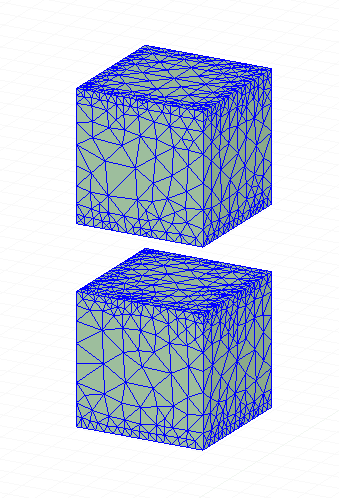
\includegraphics[width=0.5\linewidth]{p4/p4FIG3}
%    \vspace{-4mm}\caption{The mesh generated by ANSYS Maxwell after 25 passes of automatic mesh refinement for the magnetic configuration shown in Figure \ref{fig:p4cubeMagnetsRepulsion}. This mesh uses approximately 58,000 tetrahedral elements with quadratic shape functions, with approximately 4,500 elements per magnet and 49,000 elements in the region between and around the magnets.}
%    \label{fig:p4cubeMesh}
%\end{figure}
\begin{figure}
    \centering
    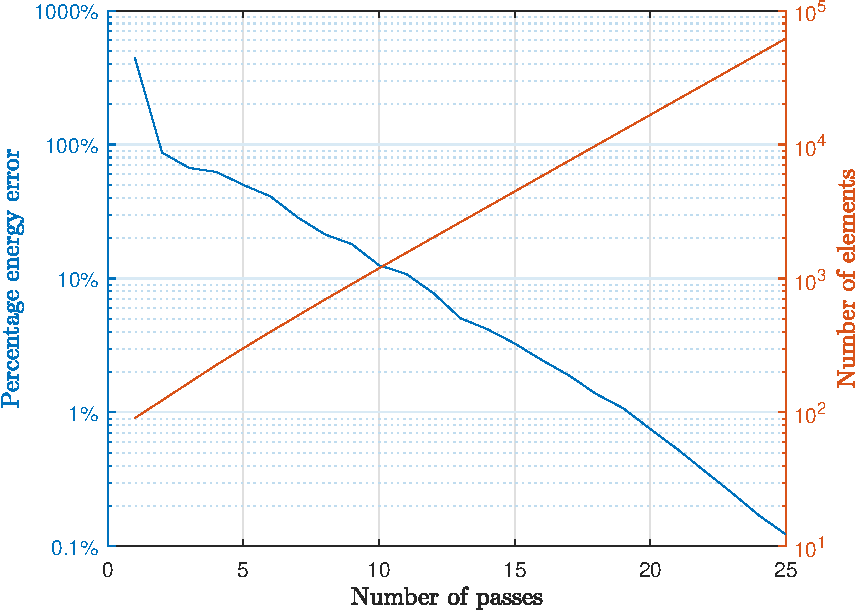
\includegraphics[width=0.8\textwidth]{p4/p4FIG4}
    \caption{Percentage energy error and number of tetrahedral elements in the ANSYS Maxwell simulation for \(d = 0.5\) as the number of passes of automatic mesh generation is increased.}
    \label{fig:p4repulseConvergence}
\end{figure}
\begin{figure}
	\centering
	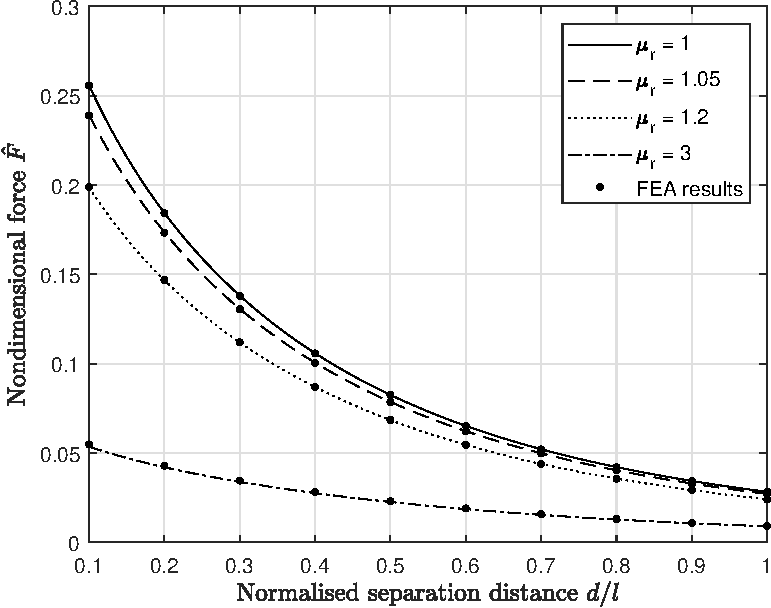
\includegraphics[width=0.8\linewidth]{p4/p4FIG5}
	\caption{Nondimensionalised force between the two magnets in Figure \ref{fig:p4cubeMagnetsRepulsion} for \(\mu_r = 1\) (calculated using \cite{Akoun1984}), \(\mu_r = 1.05\), \(\mu_r = 1.2\), and \(\mu_r = 3\). The forces calculated using the methodology presented in this paper are denoted with lines, with finite element simulations represented with large dots. The methodology presented above is in strong agreement with the finite element simulations, indicating correct force results.}
	\label{fig:p4cubeMagnetForces}
\end{figure}

In this simple repulsion configuration, it can be seen in Figure \ref{fig:p4cubeMagnetForces} that modelling neodymium magnets with \(\mu_r = 1\) overestimates the force by at least 4\%. While this is a nontrivial error, it is often accurate enough for preliminary designs. However, more permeable magnetic materials may give considerably larger errors. For this configuration, modelling hard ferritic magnets and alnico magnets with \(\mu_r = 1\) overestimates the force by at least 17\% and 170\% respectively. Thus, consideration of relative permeability in magnetostatic analysis is of high importance in electromagnetic design.

\subsection{Rotated magnets}
To verify the calculation of torque, a similar example is presented. Two cuboidal magnets, shown in Figure \ref{fig:p4cubeMagnetsRotated}, are positioned with a distance of \(3l/2\) between their centres. Initially, both magnets are parallel and magnetised along the positive vertical direction. The bottom magnet is rotated about its centre, and the force and torque on the magnet evaluated as it is rotated. The forces are nondimensionalised using Equation (\ref{eqn:p4forceNormalisation}) and the torques nondimensionalised by
\begin{equation}
	\hat{T} = \frac{\mu_0}{l^3 B_{r\text{,top}} B_{r,\text{bot}}} T \text{.}
\end{equation}
In addition, finite element simulations were conducted to examine error in the solutions found using this methodology. After 25 passes, the finite element mesh was similar to that obtained in Section \ref{sec:p4verification:magnetsRepulsion}, using approximately 58,000 tetrahedral elements, with approximately 4,500 elements per magnet and 49,000 elements in the region between and around the magnets. The percentage energy error and number of tetrahedral elements for \(\theta =\ \)\ang{60} at each pass is shown in Figure \ref{fig:p4rotateConvergence}, indicating convergence in the simulations. The torque results are plotted in Figure \ref{fig:p4cubeMagnetRotatedTorquex}, with the force results in Figures \ref{fig:p4cubeMagnetRotatedForcey} and \ref{fig:p4cubeMagnetRotatedForcez}.
\begin{figure}
	\centering
	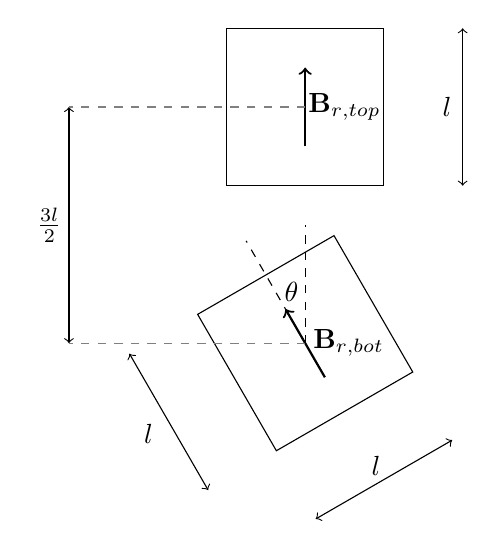
\begin{tikzpicture}

% Set up coordinates of vertices
\coordinate(toptl) at (-1,4);
\coordinate(toptr) at (1,4);
\coordinate(topbl) at (-1,2);
\coordinate(topbr) at (1,2);
\coordinate(bottl) at (0.366,1.366);
\coordinate(bottr) at (-1.366,0.366);
\coordinate(botbl) at (1.366,-0.366);
\coordinate(botbr) at (-0.366,-1.366);

% Draw magnets
\draw (toptl) -- (toptr) -- (topbr) -- (topbl) -- cycle;
\draw (bottl) -- (bottr) -- (botbr) -- (botbl) -- cycle;

% Draw magnetisation vectors
\draw[->,thick] (0,2.5) -- (0,3.5);
\draw[->,thick] (0.25,-0.433) -- (-0.25,0.433);
\node(Mtop) at (0.5,3) {\(\mathbf{B}_{r\text{,top}}\)};
\node(Mbot) at (0.55,-0) {\(\mathbf{B}_{r\text{,bot}}\)};

% Draw centres
%\node(ctop) at (0,4) {\textbf{.}};
%\node(cbot) at (0,0) {\textbf{.}};

% Draw dimensions
\draw[<->] (2,2) -- (2,4);
\node(lsidetop) at (1.8,3) {\(l\)};
\draw[<->] (-2.232,-0.134) -- (-1.232,-1.866);
\node(lsidebot) at (-1.99,-1.15) {\(l\)};
\draw[<->] (1.866,-1.232) -- (0.134,-2.232);
\node(lunder) at (0.9,-1.559) {\(l\)};
\draw[<->] (-3,0) -- (-3,3);
\node(d) at (-3.25,1.5) {\(\frac{3l}{2}\)};

% Draw horizontal centrelines
\draw[dashed,gray] (0,3) -- (-3,3);
\draw[dashed,gray] (0,0) -- (-3,0);

% Draw angle
\draw[dashed] (0,0) -- (0,1.5);
\draw[dashed] (0,0) -- (-0.75,1.3);
\node(theta) at (-0.175,0.65) {\(\theta\)};

\end{tikzpicture}
	\caption{Two cube magnets with a side length of \(l\) maintaining a constant distance of \(3l/2\) between their centres. The force and torque on the bottom magnet is calculated as it is rotated an angle \(\theta\) about its centre.}
	\label{fig:p4cubeMagnetsRotated}
\end{figure}
\begin{figure}
    \centering
    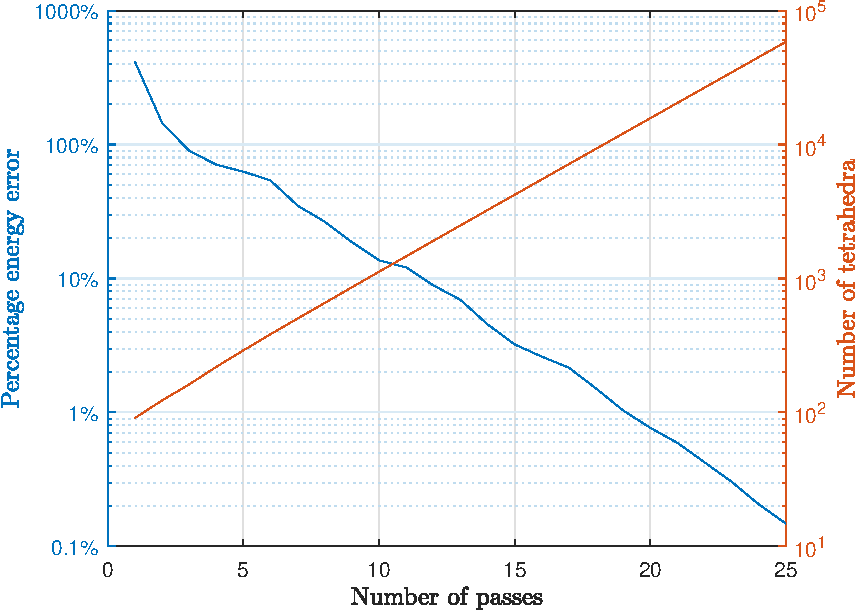
\includegraphics[width=0.8\linewidth]{p4/p4FIG7}
    \caption{Percentage energy error and number of tetrahedral elements in the ANSYS Maxwell simulation for \(\theta =\ \)\ang{60} as the number of passes of automatic mesh generation is increased.}
    \label{fig:p4rotateConvergence}
\end{figure}
\begin{figure}
	\centering
	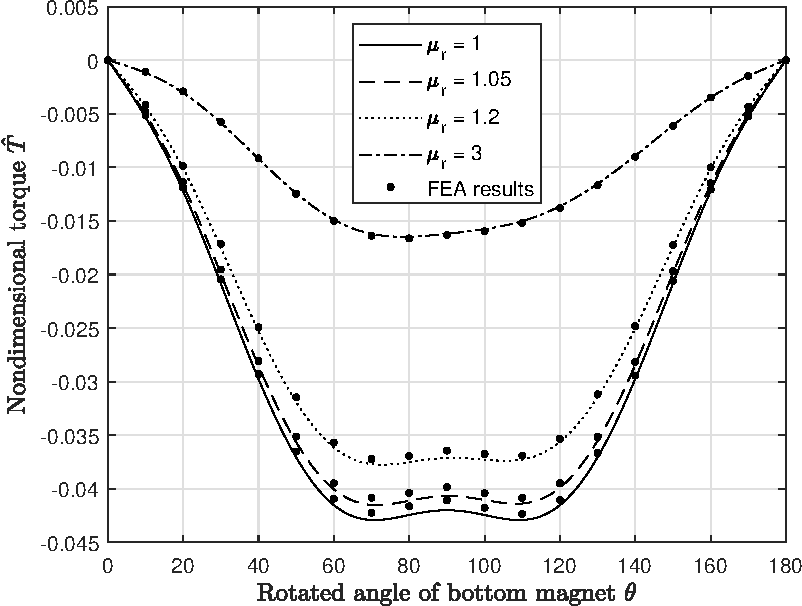
\includegraphics[width=0.8\linewidth]{p4/p4FIG8}
	\caption{Nondimensional torque on the bottom magnet about the axis of rotation of the magnet as it rotates for varying relative permeabilities \(\mu_r\). Finite element results are depicted with large dots, indicating some agreement with the results using the above methodology, with the FEA results being approximately 2\% smaller in magnitude for low permeabilities.}
	\label{fig:p4cubeMagnetRotatedTorquex}
\end{figure}
\begin{figure}
	\centering
	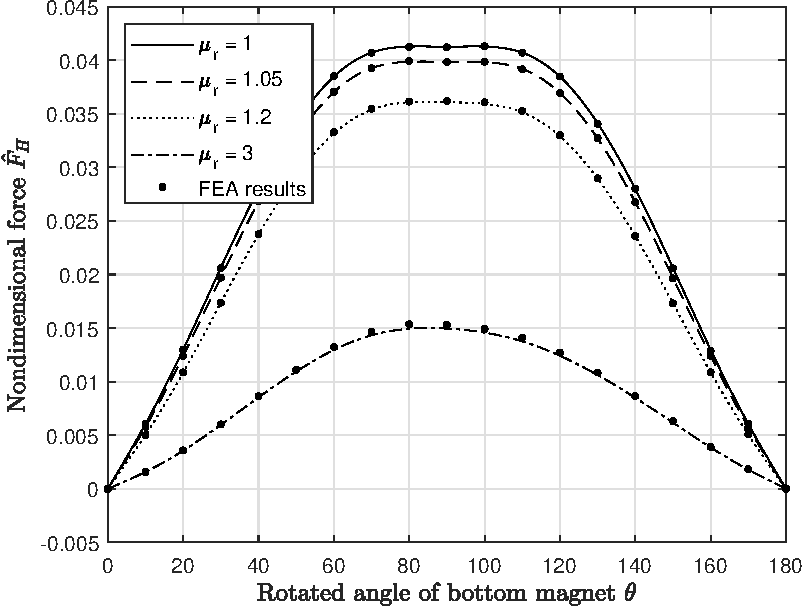
\includegraphics[width=0.8\linewidth]{p4/p4FIG9}
	\caption{Nondimensional horizontal force \(F_H\) on the bottom magnet as it rotates for varying relative permeabilities \(\mu_r\). Finite element results are depicted using large dots, indicating strong agreement with the results using the above methodology.}
	\label{fig:p4cubeMagnetRotatedForcey}
\end{figure}
\begin{figure}
	\centering
	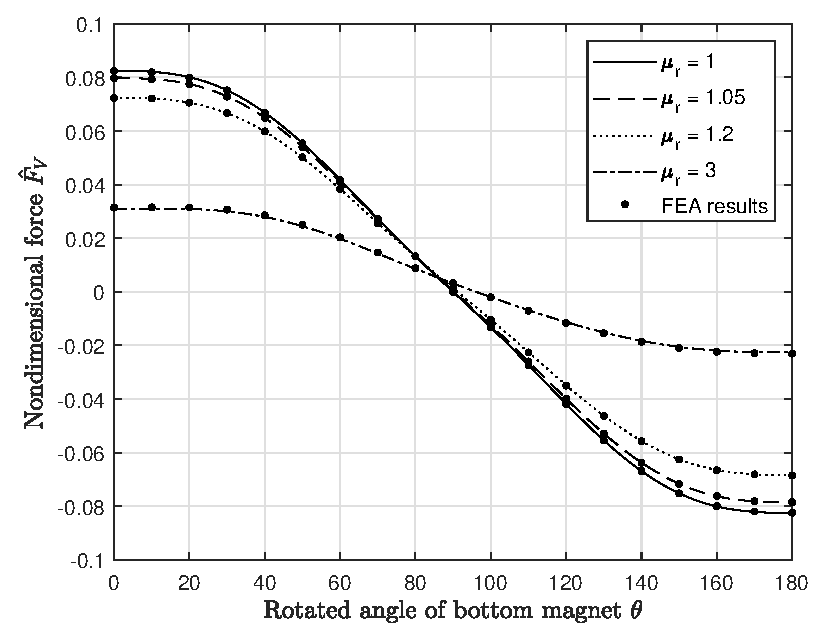
\includegraphics[width=0.8\linewidth]{p4/p4FIG10}
	\caption{Nondimensional vertical force \(F_V\) on the bottom magnet as it rotates for varying relative permeabilities \(\mu_r\). Finite element results are depicted using large dots, indicating strong agreement with the results using the above methodology.}
	\label{fig:p4cubeMagnetRotatedForcez}
\end{figure}
Figures \ref{fig:p4cubeMagnetRotatedTorquex}, \ref{fig:p4cubeMagnetRotatedForcey}, and \ref{fig:p4cubeMagnetRotatedForcez} show that the results obtained match closely with the finite element data. A small error between the estimated and FEA force results can be seen, with a larger error between the estimated and FEA torque results. To determine the source of this error, a special case of this configuration was used by setting \(\theta =\ \)\ang{90} and \(\mu_r = 1\). Since the magnets have parallel faces and a relative permeability of unity in this particular case, equations published by \textcite{Akoun1984} and \textcite{Janssen2010} can be used to calculate the exact force and torque respectively. The exact force in the horizontal direction and torque about the axis of rotation were calculated and compared to the results obtained using the methodology in this paper and finite element results, and are shown in Table \ref{tab:p4analyticTorque}.
\begin{table*}
    \centering
    \begin{tabular}{l|cc|cc}
    Method & $\hat F_H$ & Error & $\hat T$ & Error \\
    \hline
    Exact [4], [8] & $-0.04127$ & --- & $-0.04200$ & --- \\
    This work & $-0.04126$ & $0.02\%$ & $-0.04201$ & $0.24\%$ \\
    FEA & $-0.04120$ & $0.17\%$ & $-0.04107$ & $2.20\%$ \\
    \end{tabular}
    \caption{Nondimensional horizontal force \(\hat{F}_H\) and torque about the axis out of the page \(\hat{T}\) on the bottom magnet in Figure \ref{fig:p4cubeMagnetsRotated} at an angle of \ang{90} with both magnets having a relative permeability of \(\mu_r = 1\). The work presented here uses approximately 6,000 triangular surface elements, whereas the finite element simulations use approximately 58,000 tetrahedral volume elements. The work presented here has a considerably smaller percentage error than the finite element results when compared to the exact analytic results \cite{Akoun1984,Janssen2010}, indicating high accuracy of the work presented in this paper.}
    \label{tab:p4analyticTorque}
\end{table*}
It can be seen that for both force and torque, the results obtained using this methodology are considerably more accurate than the finite element results, with a percentage error almost ten times smaller. It appears that the finite element results are underestimating the force and torque, which may explain the discrepancy in Figures \ref{fig:p4cubeMagnetRotatedTorquex}, \ref{fig:p4cubeMagnetRotatedForcey}, and \ref{fig:p4cubeMagnetRotatedForcez}.

Interestingly, Figures \ref{fig:p4cubeMagnetRotatedTorquex}, \ref{fig:p4cubeMagnetRotatedForcey}, and \ref{fig:p4cubeMagnetRotatedForcez} show asymmetry when \(\mu_r \neq 1\). This is particularly visible in Figure \ref{fig:p4cubeMagnetRotatedTorquex} when \(\mu_r = 3\) between \(\theta =\ \)\ang{60} and \(\theta =\ \)\ang{120}, but this asymmetry occurs in all three plots and becomes more apparent as \(\mu_r\) is increased. This asymmetry is a result of the magnets producing fields which either strengthen or weaken the magnetisation of the other. When \(\theta <\ \)\ang{90}, the vertical component of the net field produced by the bottom magnet on the surface of the top magnet is in the same direction as \(\mathbf{B}_{r\text{,top}}\), thus strengthening the magnetisation of the top magnet. In the same way, the top magnet produces a field which strengthens the magnetisation of the bottom magnet. However, when \(\theta >\ \)\ang{90}, the opposite is true: Each magnet produces a field which weakens the magnetisation of the other magnet. Thus, each magnet strengthens the magnetisation of the other for \(\theta <\ \)\ang{90} and weakens the magnetisation of the other for \(\theta >\ \)\ang{90}, resulting in an asymmetry across \(\theta =\ \)\ang{90}, with a smaller magnitude of force and torque on the right side of each plot and a larger magnitude on the left.

In addition to verifying the force and torque, the magnetic field calculation is verified using the magnetic configuration in Figure \ref{fig:p4cubeMagnetsRotated} with \(\theta =\ \)\ang{90} and \(\mu_r = 3\) (as seen in Figure \ref{fig:p4cubeMagnetRotatedImage}). The magnetic field strength was calculated on the plane between the two magnets using the methodology in Section \ref{sec:p4magneticField} and nondimensionalised by the remanence magnetisation \(B_r\). In addition, finite element simulations were conducted on the same system using ANSYS Maxwell. The magnetic field strength computed using Section \ref{sec:p4magneticField} is plotted in Figure \ref{fig:p4cubeMagnetRotatedField}, along with the magnetic field strength generated by finite element simulations. The error is negligible, with a maximum error of 0.3\% of the remanence magnetisation, indicating the methodology used is calculating magnetic fields accurately.
\begin{figure}
	\centering
	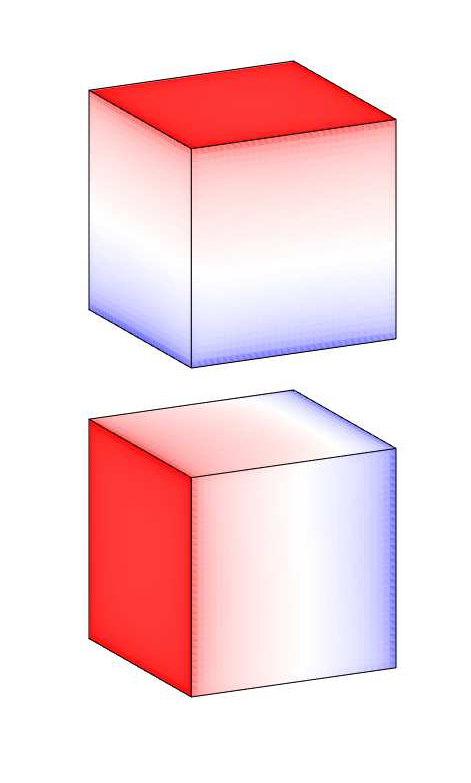
\includegraphics[width=0.55\linewidth]{p4/p4FIG11}
	\caption{The surface charge densities of the magnets in Figure \ref{fig:p4cubeMagnetsRotated} when \(\theta =\ \)\ang{90} and \(\mu_r = 3\). Due to the relatively large permeability, the top surface of the bottom magnet has considerably more positive surface charges accumulating than negative charges.}
	\label{fig:p4cubeMagnetRotatedImage}
\end{figure}
\begin{figure}
	\centering
	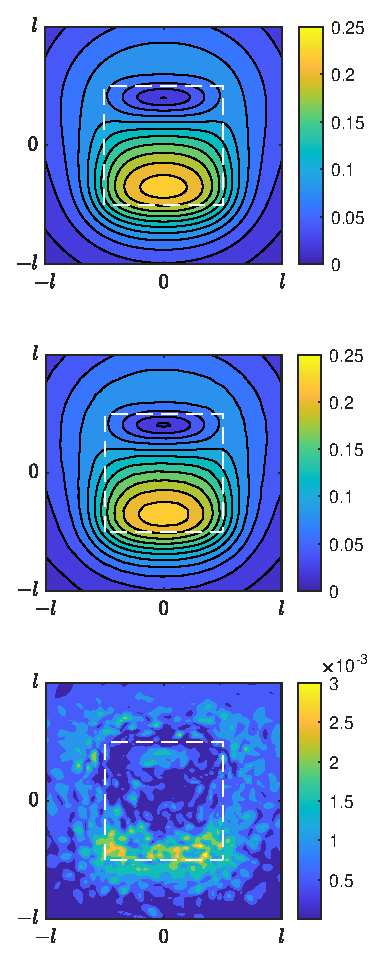
\includegraphics[width=0.5\linewidth]{p4/p4FIG12}
	\caption{The magnetic field strength \(\left| \mathbf{B} \right|\) normalised by \(B_r\) on the plane between the two magnets in Figure \ref{fig:p4cubeMagnetsRotated} when \(\theta =\ \)\ang{90}. The projections of the magnets onto the plane are displayed using white dashed lines. The field was calculated using the methodology in this paper (top) and finite element simulations (middle), with the absolute error between the two calculated (bottom). This shows strong agreement, with a maximum error of 0.3\% of the remanence magnetisation.}
	\label{fig:p4cubeMagnetRotatedField}
\end{figure}
\section{Computational performance}\label{sec:p4computationalPerformance}
In contrast to other methods, this methodology has been designed in such a way that the magnetic field \(\mathbf{B}\) needs to be calculated only once, but requires the inversion of a potentially large non-sparse matrix (performed using the backslash operator or \texttt{mldivide} function in MATLAB). As such, it is considerably faster than the iterative methods often seen in literature, but requires more computational memory. In addition, this method uses an analytical equation \cite{OConnell2020a} to calculate the magnetic field, making it faster than finite element methods to obtain an accurate solution.

\subsection{Computational speed}
To assess computation speed, a simple magnetic system was defined using two cube magnets in repulsion, separated by one magnet width, equivalent to Figure \ref{fig:p4cubeMagnetsRepulsion} with \(d = l\). To assess accuracy, the relative permeability of the magnets was set to unity, \(\mu_r = 1\), which allows the use of exact analytic force equations published by \textcite{Akoun1984}. The force was calculated using both the methodology defined in this paper, finite element simulations, and the exact force equations using MATLAB R2020a on a personal computer with an Intel Xeon E3-1240 v5 at 3.50GHz with 16GB of memory. The force calculations using finite element simulations and the methodology in this paper were repeated with varying mesh densities and timed to give an indication of computation speed. Both methods were compared to the exact analytic force equations \cite{Akoun1984} to give a measure of error, with both methods showing approximately the same rate of error convergence, but with the methodology in this paper giving results approximately an order of magnitude faster for the same accuracy. The percentage error between the estimated force using the method in this paper and exact force was computed and is displayed in Figure \ref{fig:p4calculationTime}.
\begin{figure}
	\centering
	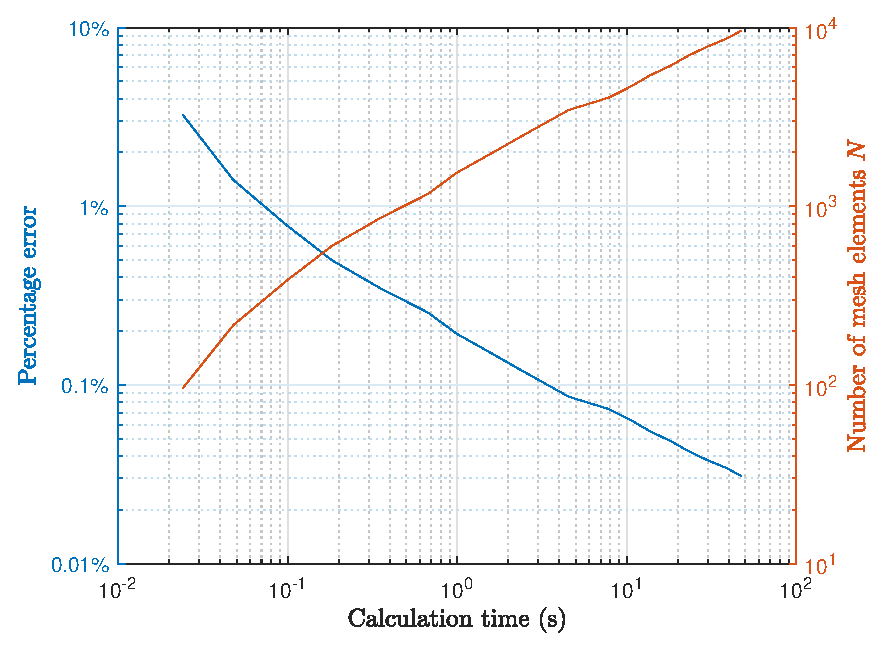
\includegraphics[width=0.8\linewidth]{p4/p4FIG13}
	\caption{Percentage error in the calculation of vertical force \(F_V\) between the magnets shown in Figure \ref{fig:p4cubeMagnetsRepulsion} with \(d = l\) and \(\mu_r = 1\) as mesh density, and thus calculation time, is increased. The number of surface mesh elements \(N\) is also plotted, showing an inverse trend when compared to the percentage error.}
	\label{fig:p4calculationTime}
\end{figure}

As expected, the percentage error decreases as calculation time increases. For this particular magnetic configuration and computation hardware, finite element simulations generally took more than 5s to achieve an error within 1\%. In contrast, the methodology in this paper took less than 100ms to attain less than 1\% error and less than 5s to attain less than 0.1\% error. This will vary depending on magnetic configuration, code implementation, and computation hardware, but gives an indication of the expected order of magnitude of calculation time to achieve a desired accuracy.

\subsection{Memory requirements}
This methodology requires more computational memory than other methods found in literature. Iterative methods, for example, require enough memory to keep track of the surface charge densities, but must recalculate the magnetic field information at each step. This can be done using a single \(N\times 1\) vector. In contrast, this method requires storing several large \(N\times N\) matrices of floating point numbers, as well as enough memory to invert a large \(\left(N+M\right) \times \left(N+M\right)\) matrix. This is a significantly larger memory requirement than iterative methods, but results in a considerably faster solution. During testing by the authors, a high precision calculation may use more than one gigabyte of memory, with equivalent finite element simulations requiring tens of gigabytes of memory. While considerable memory requirements are necessary for the method outlined in this paper, mesh optimisation was not considered. As such, testing was done using a basic mesh, with all elements being similar in size. If a more appropriate mesh is chosen, with finer mesh in areas with large magnetic field gradient, a high precision calculation can be done using less memory.

\subsection{Meshing considerations}
In this paper, a surface mesh has been used under the assumption that the magnetic permeability and remanence magnetisation vector are constant and uniform. If these assumptions are not valid, a volume mesh may be used and a similar methodology applied, where the magnetisation vector of each volume element is computed rather than the scalar surface charge density. However, the use of a volume mesh rather than surface mesh comes with a more considerable computation cost. Solving for the magnetisation vector field requires solving a large linear equation for each of the three Cartesian directions, while the scalar surface charge density solution only requires a single linear equation. In addition, calculation of the field produced by each element would require either using an inaccurate point dipole model, or calculating the field contribution from each of the surfaces of the element \cite{OConnell2020,OConnell2020a}. The use of the point dipole model considerably decreases accuracy for nearby elements, and the more complicated method considerably increases calculation time. These factors lead to a significantly larger computation cost when applying a volume mesh and solving the magnetisation vector field. Thus, for systems with constant and uniform permeability and remanence magnetisation, a surface charge density approach is preferred.

The methodology in this work uses a triangular surface mesh generated by finding the minimum convex hull of a set of vertices using the Geom3D library in the MatGeom package in MATLAB \cite{Legland2021}. Subdivision of the surface mesh is performed by dividing each triangular element into four congruent triangles until a desired number of surface elements was achieved. A triangular surface mesh has been chosen since analytic field equations are available for these elements \cite{OConnell2020a,OConnell2020}. These equations may be used to solve for the field produced by a triangle with constant surface charge density, and are highly efficient, especially when many field calculations are performed. In addition, a triangular surface mesh can represent any polyhedral surface and can be used to approximate curved surfaces, enabling the approximate solution of any magnetic configuration. The meshing algorithm itself is out of the scope of this work, since it is focused only on calculating the charge densities on each surface element and the resulting fields, forces, and torques. However, alternative meshing algorithms may be applied, and future analysis could be done on optimising the meshing process for this methodology.

\section{Conclusion}\label{sec:p4conclusion}
This paper has outlined a new algorithm for modelling magnetic materials with nonunity relative permeability. Assuming constant uniform magnetisation and constant permeability, the algorithm uses a one-step matrix inversion to solve for the surface charge density, magnetic field, force, and torque. In contrast to other methods available in literature, this method calculates magnetic field information only once, leading to a considerable increase in calculation speed. In addition, using a triangular surface mesh gives this methodology high versatility, allowing the modelling of any polyhedral magnet, and approximate modelling of any general magnet geometry.

The algorithm was verified against literature and finite element simulations using several magnetic configurations. A simple magnetic configuration was defined with two cube magnets in repulsion with varying permeabilities, with the force between the magnets calculated. The force results showed strong agreement with finite element simulations. In addition, it was shown that the permeability has a significant effect on the force between the magnets, and as such, care must be taken when assuming a relative permeability of unity. A similar magnetic configuration was used to verify the torque, where the magnets maintain a constant distance between their centres, but one magnet is rotated. The torque results were in agreement with finite element simulations, and it was again shown that permeability greatly affects torque. Furthermore, the magnetic field was calculated on the plane between the magnet centres with \(\theta =\ \)\ang{90}. Finite element simulations showed strong agreement, with a negligible error.

This methodology has allowed fast and accurate results for any magnet geometry and configuration. This can be used for fast optimisation of electromagnetic designs, giving more accurate results than analytic methods which assume unity relative permeability, and faster results than finite element simulations.
\begin{subappendices}
\addcontentsline{toc}{section}{\protect\numberline{}Appendices}
\addtocontents{toc}{\protect\setcounter{tocdepth}{-1}}
\renewcommand{\thesection}{Appendix \arabic{chapter}.\Alph{section}}
\section{Volume charge density}\label{sec:p4noVolumeCharge}
Consider a magnetic material with constant permeability \(\mu_r\) and constant uniform remanence magnetisation \(\mathbf{B}_r\). According to Equation (\ref{eqn:p4equivalentMagnetisation}), this material will satisfy the equation
\begin{equation}
    \mathbf{M} = \frac{\mu_r - 1}{\mu} \mathbf{B} + \frac{1}{\mu} \mathbf{B}_r \text{.}
\end{equation}
To calculate the volume charge density \(\nabla \cdot \mathbf{M}\), take the divergence of both sides, giving
\begin{equation}
    \nabla \cdot \mathbf{M} = \nabla \cdot \left( \frac{\mu_r - 1}{\mu} \mathbf{B} \right) + \nabla \cdot \left( \frac{1}{\mu} \mathbf{B}_r \right) \text{.}
\end{equation}
However, under the assumption of constant permeability, the permeability terms can be taken out of the divergence,
\begin{equation}\label{eqn:p4divM}
    \nabla \cdot \mathbf{M} = \frac{\mu_r - 1}{\mu} \nabla \cdot \mathbf{B} + \frac{1}{\mu} \nabla \cdot \mathbf{B}_r \text{.}
\end{equation}
Maxwell's equations state that the \(\mathbf{B}\) field is solenoidal, \(\nabla \cdot \mathbf{B} = 0\). In addition, the assumption of constant uniform remanence magnetisation leads to \(\nabla \cdot \mathbf{B}_r = 0\). Consequently, the right side of Equation (\ref{eqn:p4divM}) becomes zero, and therefore
\begin{equation}
    \nabla \cdot \mathbf{M} = 0 \text{.}
\end{equation}
Thus, a material with constant uniform remanence magnetisation and constant permeability has no volume charge density and the volume integral for the charge method may be neglected.
\section{Matrix invertibility}\label{sec:p4invertibleMatrix}
Consider the system defined by the matrix equation
\begin{equation}\label{eqn:p4invertibleProofEquation}
    C \bm{\sigma} = K \bm{\sigma}_0 \text{,}
\end{equation}
where \(C\) is an \(N\times N\) square matrix and \(\bm{\sigma}\) and \(\bm{\sigma}_0\) are \(N\times 1\) vectors of final and initial surface charge densities respectively. This section will show that the matrix \(C\) is invertible using contradiction.

Suppose \(C\) has at least one eigenvalue equal to zero, \(\lambda = 0\). This implies that there exists a \textit{non-zero} eigenvector \(\bm{\sigma}\) of \(C\) such that
\begin{equation}
    C\bm{\sigma} = \lambda \bm{\sigma} = 0 \bm{\sigma} = \mathbf{0} \text{.}
\end{equation}
Substituting this into Equation (\ref{eqn:p4invertibleProofEquation}) leads to
\begin{equation}
    K \bm{\sigma}_0 = \mathbf{0} \text{.}
\end{equation}
Since \(\mu_r\) is a finite positive value for the magnetic materials considered in this work, \(K \neq 0\), and thus,
\begin{equation}
    \bm{\sigma}_0 = \mathbf{0} \text{.}
\end{equation}
We know that \(\bm{\sigma} \neq \mathbf{0}\) by the definition of an eigenvector. Thus, this implies that there exists a system with zero initial magnetic charge density, \(\bm{\sigma}_0 = \mathbf{0}\), which becomes spontaneously magnetised, such that \(\bm{\sigma} \neq \mathbf{0}\), with no external field. This is clearly absurd, and the assumption of any eigenvalues being equal to zero fails. Thus, all eigenvalues of \(C\) must be nonzero and therefore \(C\) must be invertible.

While \(C\) is invertible, it may have an undesirable condition number, leading to errors when inverting. However, this method uses constrained least squares, and \(C\) is never directly inverted; it is simply shown here to be invertible to imply a solution for \(\bm{\sigma}\) exists.
\section{Surface charge density over a magnet}\label{sec:p4integralSigma}
Taking the divergence of Equation (\ref{eqn:p4equivalentMagnetisation}) inside the volume \(V\) of a magnetic body gives
\begin{equation}
    \nabla \cdot \mathbf{M} = \nabla \cdot \left( \frac{\mu_r-1}{\mu} \mathbf{B} \right) + \nabla \cdot \left( \frac{1}{\mu} \mathbf{B}_r \right) \text{.}
\end{equation}
Assuming the permeability \(\mu\) is constant (and thus \(\mu_r\) is also constant), the permeability terms may be taken out of the divergence operators,
\begin{equation}
    \nabla \cdot \mathbf{M} = \frac{\mu_r-1}{\mu} \nabla \cdot \mathbf{B} + \frac{1}{\mu} \nabla \cdot \mathbf{B}_r \text{.}
\end{equation}
However, we know that \(\mathbf{B}\) is divergence-free from Maxwell's equations. In addition, we are assuming that the remanence magnetisation inside the volume \(V\) is constant and uniform, implying it is also divergence-free. Therefore, inside the volume of a magnet, \(\nabla \cdot \mathbf{B} = 0\) and \(\nabla \cdot \mathbf{B}_r = 0\), and
\begin{equation}
    \nabla \cdot \mathbf{M} = 0 \text{.}
\end{equation}
We can then take the volume integral of this expression inside the volume \(V\), giving
\begin{equation}
    \iiint_V \nabla \cdot \mathbf{M}\ dv = 0 \text{.}
\end{equation}
Finally, since \(\mathbf{M}\) is assumed to be well-behaved inside the magnet, we can apply the divergence theorem to the integral, giving
\begin{equation}
    \oiint_S \mathbf{M} \cdot \hat{\mathbf{n}}\ ds = 0 \text{.}
\end{equation}
Since the surface charge density is given by \(\sigma = \mathbf{M} \cdot \hat{\mathbf{n}}\), we finally obtain
\begin{equation}\label{eqn:p4integralSigma}
    \oiint_S \sigma \ ds = 0 \text{.}
\end{equation}
\end{subappendices}
\clearpage
\section*{Author's remarks on Chapter \ref{chap:paper4}}
This chapter presents the final article submitted in this thesis, and successfully modelled permanent magnets with non-unity relative permeability using a semi-analytic approach. While this method is fast and highly accurate, it does require the assumption of constant permeability, and is unable to accurately model non-linear magnetic materials. However, permanent magnets are generally highly linear in their operating regions, and as such this method models them accurately. While the approaches seen in Chapters \ref{chap:paper1} and \ref{chap:paper2} are considerably faster to evaluate than this method, they cannot model non-unity relative permeability and will see several percentage points of error when modelling real permanent magnets. This method is slower, but far more accurate, and when combined with the field equations from Chapter \ref{chap:paper2}, can accurately model any permanent magnet of any shape.
\addtocontents{toc}{\protect\setcounter{tocdepth}{2}}

\newpage
\section*{References}
\addcontentsline{toc}{section}{\protect\numberline{}References}
\printbibliography[heading=none]